\begin{figure}[H]
	\centering
	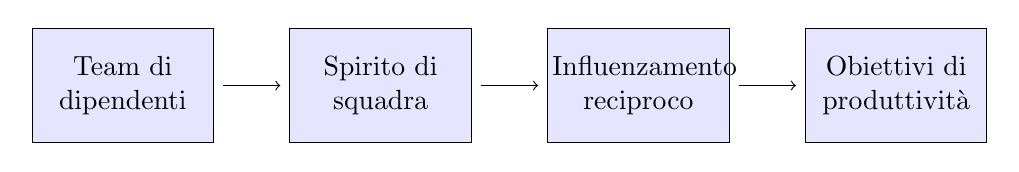
\begin{tikzpicture}
		\draw[fill=blue,fill opacity=0.1] (0,0) rectangle ++(0.19\textwidth,0.12\textwidth);
		\draw (0,0) rectangle ++(0.19\textwidth,0.12\textwidth)
		node[pos=.5, text width=0.18\textwidth, align=center] {Team di dipendenti};
		\draw[->] (0.20\textwidth,0.06\textwidth) -- (0.26\textwidth,0.06\textwidth);
		\draw[fill=blue,fill opacity=0.1] (0.27\textwidth,0) rectangle ++(0.19\textwidth,0.12\textwidth);
		\draw (0.27\textwidth,0) rectangle ++(0.19\textwidth,0.12\textwidth)
		node[pos=.5, text width=0.18\textwidth, align=center] {Spirito di squadra};
		\draw[->] (0.47\textwidth,0.06\textwidth) -- (0.53\textwidth,0.06\textwidth);
		\draw[fill=blue,fill opacity=0.1] (0.54\textwidth,0) rectangle ++(0.19\textwidth,0.12\textwidth);
		\draw (0.54\textwidth,0) rectangle ++(0.19\textwidth,0.12\textwidth)
		node[pos=.5, text width=0.18\textwidth, align=center] {Influenzamento reciproco};
		\draw[->] (0.74\textwidth,0.06\textwidth) -- (0.80\textwidth,0.06\textwidth);
		\draw[fill=blue,fill opacity=0.1] (0.81\textwidth,0) rectangle ++(0.19\textwidth,0.12\textwidth);
		\draw (0.54\textwidth,0) (0.81\textwidth,0) rectangle ++(0.19\textwidth,0.12\textwidth)
		node[pos=.5, text width=0.18\textwidth, align=center] {Obiettivi di produttività};
	\end{tikzpicture}
\end{figure}
